\documentclass[11pt,a4paper]{article}
\usepackage[T1]{fontenc}
\usepackage[utf8]{inputenc}
\usepackage{lmodern,amsmath,amssymb,mathtools,graphicx,booktabs,array,longtable}
\usepackage[margin=24mm]{geometry}
\usepackage{microtype}
\usepackage{xcolor}
\usepackage{hyperref}
\usepackage{enumitem}
\hypersetup{colorlinks=true,linkcolor=blue!45!black,citecolor=blue!45!black,urlcolor=blue!45!black,pdftitle={WestQuant Memory Discovery Lab},pdfauthor={David Vesterlund}}
\setlength{\emergencystretch}{2em}
\setlength{\parskip}{3pt}
\makeatletter\setlength{\@fptop}{0pt}\makeatother
\newcommand{\Tr}{\operatorname{Tr}}
\newcommand{\E}{\mathcal E}
\newcommand{\D}{\mathcal D}
\newcommand{\ket}[1]{\lvert #1\rangle}
\newcommand{\bra}[1]{\langle #1\rvert}
\newcommand{\code}[1]{\texttt{#1}}
\title{WestQuant Memory Discovery Lab:\\An Evidence-Aware Framework from Experimental Data to Quantum-Memory Simulation}
\author{David Vesterlund\\\small WestQuant, Vesterlund Ventures, Sweden\\\small Independent research program}
\date{10 October 2026}
\begin{document}
\maketitle
\begin{abstract}
Quantum-memory modeling requires more than a material coherence time: the measured observable, pulse protocol, temperature, optical transfer and conditional acceptance must be specified together. We present WestQuant Memory Discovery Lab, a Python framework linking versioned source artifacts to typed observations, reviewed coherence references, deterministic dynamical models and optional network-channel export. Its contribution is the executable integration and its explicit limits of inference, rather than a new microscopic theory. A fresh reanalysis of 90 released state-fidelity values from a Pr$^{3+}$:Y$_2$SiO$_5$ memory array recovers path and time-bin means of 0.951082 and 0.914048. A within-dataset spatial holdout has a maximum standardized discrepancy of 2.342 under the stated uncertainty approximation. Eight decay fits to a separate open Pr-memory dataset produce six model mismatches and two inconclusive results; none identifies a homogeneous spin $T_2$. Analytical spin-bath controls and a synthetic count experiment verify the deterministic and inference branches, while 75 automated tests pass. An experimentally constrained, nonunique operating-point channel is propagated through SeQUeNCe: 87 pairs are retrieved in 400,000 ideal-input attempts, consistent with its fixed-loss model. These network outcomes are simulations, not experimental entanglement measurements. The framework retains ten reviewed coherence references and 201 provisional molecular observations without converting incomplete labels into physical predictions. The results establish a reproducible data-to-simulation workflow within declared model domains; they do not establish a new material or improved hardware performance.
\end{abstract}
\noindent\textbf{Keywords:} quantum memories; reproducible simulation; provenance; open experimental data; spin coherence; quantum channels; quantum networks.

\section{Introduction}
The useful lifetime of a quantum memory depends on the task being performed. Spin coherence, optical coherence, storage efficiency and conditional qubit fidelity are different observables. A material may preserve a spin superposition under a specialized pulse sequence while lacking an efficient or sufficiently quiet optical write/read interface. Consequently, a numerical value labeled $T_2$ cannot by itself determine whether a device supplies useful states to a quantum network.

Published experiments illustrate these distinctions. Teller et al. demonstrated individually addressable memory cells and measured path- and time-bin-qubit fidelities with weak coherent probes~\cite{teller}. Ortu et al. reported protocol-dependent effective spin-coherence times together with time-bin storage~\cite{ortu}. A recent Pr-memory experiment distinguishes extended classical echoes from nonclassical heralded-photon storage~\cite{rodriguez}. Molecular-qubit studies supply complementary information about phase memory and chemical environments~\cite{lin,mullin}, whereas integrated defect experiments report distinct Ramsey and Hahn observables~\cite{hu}. These data support different model components and should not be pooled as interchangeable lifetime labels.

Existing computational tools already solve much of the relevant physics. PySCF provides electronic-structure calculations~\cite{pyscf}; PyCCE evaluates spin-bath dynamics~\cite{pycce}; QuTiP supplies open-system evolution~\cite{qutip}; and MaxwellBloch treats optical propagation~\cite{maxwellbloch}. SeQUeNCe supplies event-driven network simulation~\cite{sequence}. General workflow systems such as AiiDA address computational provenance~\cite{aiida}. Recent cross-validation of network simulators emphasizes that matching parameter names is insufficient when event and connection semantics differ~\cite{chung}. WestQuant reuses these tools. It does not replace their solvers, and the implementation evaluated here does not use AiiDA as its execution engine.

The research question is whether a common executable workflow can move from heterogeneous experimental and materials data to appropriately scoped memory simulations while retaining the evidence needed to assess each result. We address it with a typed catalog, condition-sensitive reference queries, explicit model dispatch, an acceptance-and-erasure channel contract and archived validation outputs. The same representation permits controlled candidate variations, but a generated candidate is not assumed to be a stable species or a functioning memory.

The contribution has three parts: an implemented source-to-model interface, a common memory/channel contract with declared inference boundaries, and reproducible evaluations using open experimental data and independent numerical references. Existing-memory validation supports the system contribution. Finding a better material, changing a network ranking or demonstrating a new microscopic prediction is not required for that contribution and is not claimed here. Machine learning for $T_2$ has been separated into another project and is absent from the evaluated workflow.

\section{System architecture and evidence model}
\label{sec:architecture}
Figure~\ref{fig:architecture} summarizes the implemented workflow. Each source artifact retains its URL, revision or record identifier, raw bytes, content hash, retrieval metadata and license information. Bounded downloads check source checksums when supplied. Offline execution checks the cached SHA-256 values and fails on missing or corrupted artifacts. A retrieval timestamp alone is not treated as an immutable source revision: live reference pages are frozen by their retrieved bytes and hashes.

\begin{figure}[tbp]
\centering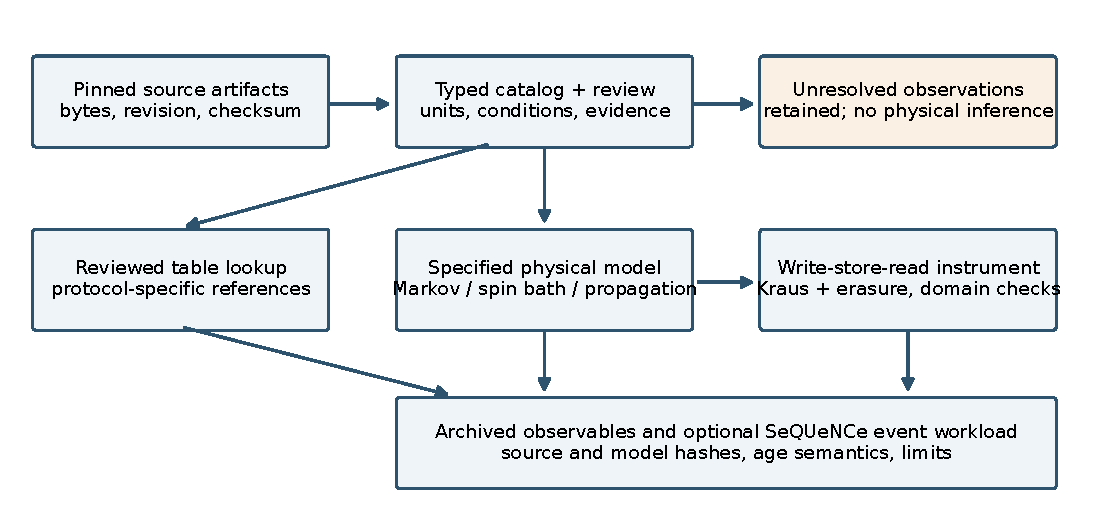
\includegraphics[width=\linewidth]{figures/architecture.pdf}
\caption{Implemented data and model boundaries. Unresolved observations remain visible in the catalog. Reviewed table values and specified physical models can produce scoped outputs; optical channel construction additionally requires write/read and loss parameters. SeQUeNCe is an optional downstream workload. A table reference is not automatically converted into a full channel.}
\label{fig:architecture}
\end{figure}

\subsection{Candidates, observations and references}
A candidate record contains elemental composition, explicit charge, electronic spin, supplied geometry, host and any site-resolved isotope substitutions. Candidate enumeration checks electron-count/spin parity and preserves the parent configuration. These checks remove inconsistent specifications; they do not establish a bound electronic state, chemical stability, accessible optical transitions or an experimentally realizable device.

An observation contains a subject identifier, quantity, value, declared unit, conditions, source location, provenance and evidence kind. Distinct kinds include experimental, curated experimental, evaluated reference, computed, hypothetical and unknown evidence. Result metadata separately records input and output evidence. For example, a computed channel constrained by a published mean remains a modeled channel rather than an experimental process-tomography result.

The catalog uses SQLite with immutable record identities. The coherence-reference extension stores a definition, a positive time in seconds, reported uncertainty convention, explicit conditions, primary-source location and unresolved conditions. Reference matching requires material identity and coherence definition, then compares the supplied reported conditions. Missing, mismatched or unverifiable conditions cannot silently yield an applicable numerical estimate. Even a reported-condition match retains the source's unresolved microscopic or operating details. No temperature, isotope, host, charge or pulse-protocol interpolation is performed by the reference-query path.

This restriction differs from the separate \emph{pure-coherence table} model: a reviewed complex-coherence curve may be interpolated linearly within its own time interval under matching temperature and control conditions. Its initial value must be unity, its magnitude must remain within the unit disk, and it must explicitly exclude population relaxation. Extrapolation is prohibited. Neither table mechanism converts a bare formula or an isotope mass into $T_2$.

\subsection{Execution and failure semantics}
Study execution enumerates configuration identities before launching bounded worker processes. Hashes include configuration and source information; random streams are derived from explicit master seeds and identities. Atomic JSON writes, checkpoints and resume logic preserve completed records. Invalid geometry, unsupported model families, missing units, incompatible temperature domains and numerical nonconvergence are failures or unresolved outcomes rather than substituted defaults. A generic study-stage gate is a workflow control, not a sufficient proof of scientific discovery; the baseline's richer discovery gate must also be interpreted at its documented scope.

The implemented dispatcher groups candidates into atomic ensembles, trapped atoms/ions, rare-earth solids, defect spins, molecular spins and a restricted negative-ion branch. This is a software taxonomy with six labels, not an exhaustive classification of quantum memories. The allowed model combinations are listed in Table~\ref{tab:branches}. Quantum dots and optomechanical devices do not have independently validated microscopic adapters in this release.

\begin{table}[tbp]
\centering\small
\begin{tabular}{p{.29\linewidth}p{.61\linewidth}}
\toprule Family or component & Implemented scope \\
\midrule
Atomic ensembles; trapped atoms/ions & Supplied Markov model or condition-matched pure-coherence table; no general first-principles device identification.\\
Rare-earth, defect and molecular spins & Above descriptions plus finite nuclear-bath evolution or conventional PyCCE coherence with supplied parameters.\\
Negative ion & Supplied Markov/table storage and a specified photodetachment environment-overlap model; no inferred bound state or coherent optical interface.\\
Electronic and propagation backends & Molecular PySCF; ORCA/QE input and coupling-import hooks; a separate MaxwellBloch propagation adapter. These do not automatically identify a memory channel.\\
Experimental operating point & A reviewed rare-earth point with exact time/protocol/temperature matching; lifetime extrapolation rejected.\\
\bottomrule
\end{tabular}
\caption{Implemented model domains. Availability of an adapter and numerical execution are separate from experimental validation of that domain.}
\label{tab:branches}
\end{table}

\section{Physical and operational model}
\label{sec:model}
\subsection{Stage-resolved conditions and Markov dynamics}
A modeled memory specifies writing, storage and reading temperatures $(T_w,T_s,T_r)$ and durations $(t_w,t,t_r)$. Each stage is isothermal in the evaluated implementation. An unspecified thermal ramp is rejected; a temperature-dependent coefficient is used only inside its declared validity interval. Phenomenological rate functions can be supplied as
\begin{equation}
\Gamma(T)=\Gamma_0+aT+b(T/T_{\rm ref})^n+
\frac{c}{\exp(\Theta/T)-1},
\label{eq:temperature}
\end{equation}
with nonnegative coefficients and an explicit reference temperature. These coefficients are inputs or calibrated model quantities. Equation~\eqref{eq:temperature} does not establish a material-specific relaxation mechanism merely because terms resemble direct, Raman or activated processes.

For stage $j$, the Markov reference uses population relaxation $\Gamma_{1,j}$, independent pure dephasing $\Gamma_{\phi,j}$, excited-state equilibrium population $p_{e,j}$ and detuning $\nu$. With $H=h\nu\ket{1}\bra{1}$ and $\mathcal L_A(\rho)=A\rho A^\dagger-\{A^\dagger A,\rho\}/2$,
\begin{align}
\dot\rho={}&-\frac{i}{\hbar}[H,\rho]
+\Gamma_1(1-p_e)\mathcal L_{\sigma_-}(\rho)
+\Gamma_1p_e\mathcal L_{\sigma_+}(\rho)
+\frac{\Gamma_\phi}{2}\mathcal L_Z(\rho),\\
\rho_{01}(t)={}&\rho_{01}(0)\exp[-(\Gamma_1/2+\Gamma_\phi)t+i2\pi\nu t].
\end{align}
Thermal detailed balance is optional and, when declared, uses a supplied qubit frequency to determine $p_e$. A separately declared activity contribution can add a phenomenological rate $\lambda a$ to storage dephasing; it is not an independently validated model of network-induced heating or pulse errors.

Under this stationary, independent-noise description,
\begin{equation}
T_1=\Gamma_1^{-1},\qquad T_2=(\Gamma_1/2+\Gamma_\phi)^{-1}.
\label{eq:t2markov}
\end{equation}
An experimentally reported \emph{total} $T_2$ must not be inserted as $\Gamma_\phi=1/T_2$ and combined with population relaxation again. The model requires an explicit rate definition to prevent this double counting. The familiar $T_2\leq 2T_1$ statement is conditional on this model and is not used as a universal filter for protocol-dependent fitted times.

\subsection{Finite nuclear-bath evolution}
Hamiltonians in the spin module are frequency operators $G$ in Hz; physical energies are $hG$. The supplied bath contains nuclear spins $I_i$, laboratory-frame Zeeman vectors $\boldsymbol\omega_i$, hyperfine tensors $A_i$, optional symmetric quadrupole tensors $Q_i$ and pair tensors $J_{ij}$:
\begin{align}
G_B={}&\sum_i\boldsymbol\omega_i\cdot\mathbf I_i+
\sum_i\sum_{ab}Q_{i,ab}I_{i,a}I_{i,b}+
\sum_{i<j}\sum_{ab}J_{ij,ab}I_{i,a}I_{j,b},\\
G_m={}&G_B+m\sum_i\sum_a A_{i,za}I_{i,a}.
\label{eq:bath}
\end{align}
The central-spin pure-dephasing approximation retains the central $S_z$ coupling and the two specified logical projections $m_0,m_1$. Transverse central-spin transitions and phonon relaxation are not generated by this approximation. Bath initialization uses
\begin{equation}
\rho_B(T)=\frac{\exp[-hG_B/(k_BT)]}{\Tr\exp[-hG_B/(k_BT)]},\qquad
L(t)=\Tr[U_0(t)\rho_B(T)U_1^\dagger(t)].
\label{eq:coherence}
\end{equation}
The zero-temperature implementation uses the normalized projector onto the numerically degenerate ground-state subspace. Free propagators contain $\exp(-i2\pi G_m\Delta t)$. Ideal CPMG pulses swap the two branch Hamiltonians at $t(j+1/2)/N$, $j=0,\ldots,N-1$. A finite Hilbert-space budget bounds exact evolution.

Conventional CCE is available through PyCCE~\cite{pycce}. Its backend units are explicitly converted: seconds to milliseconds, hyperfine Hz to kHz and field tesla to gauss. Generalized CCE density elements are not silently normalized and exported as pure coherence. Realistic predictions would additionally require bath-size, cluster-order and control-resolution convergence, which is not demonstrated for a new material in this study.

The operational descriptor returned by exact evolution is the first \emph{sampled} $1/e$ crossing of $|L|$, represented by adjacent time-grid endpoints. Revival detection and the finite observation window accompany it. This descriptor is not declared to be a unique exponential $T_2$. Absence of a sampled crossing is not proof that none occurs between samples, and is not reported as an infinite measured lifetime.

\subsection{Electronic structure, optical propagation and negative ions}
The molecular electronic adapter evaluates HF or DFT at supplied geometry, charge and spin, optionally with scalar relativistic treatment and Tamm--Dancoff excitations. Convergence is checked and recipes are included in the cache identity. A finite-basis energy does not prove an anion bound state; a vertical excitation energy does not specify $T_2$. Couplings from external calculations require explicit site mapping, tensor-frame alignment and units before entering Eq.~\eqref{eq:bath}. The evaluated workflow does not automatically calculate a complete spin--phonon spectral density from a molecular structure.

The MaxwellBloch adapter evolves a supplied multi-level optical recipe separately from the qubit-channel wrapper. It can provide propagation fields and states, but a finite-field solution is not automatically a single-photon acceptance instrument. Protocol calibration and an observable mapping remain necessary.

For photodetachment, neutralization leaves an electron or environmental record. For a modeled superposition
\begin{equation}
\ket\Psi=a\ket0\ket{E_0}+b\ket1\ket{E_1},\qquad
\rho_{01}\longmapsto\chi\rho_{01},\quad \chi=\langle E_1|E_0\rangle,
\end{equation}
tracing out that record reduces coherence unless the records overlap sufficiently. The restricted negative-ion branch therefore requires a supplied complex $\chi$ with $|\chi|\leq1$. It does not infer $\chi$ from a charge change or assert that photodetachment produces a stable quantum memory.

\subsection{Write-store-read channel and erasure}
\label{sec:instrument}
Let $\Phi_j$ be the conditional stage channel from Markov dynamics, and let $\D_z$ multiply $\rho_{01}$ by complex $z$, with $|z|\leq1$. The storage map is
\begin{equation}
\Phi_s(t)=\D_{L(t)}\circ\Phi_{s,\mathrm{Markov}}(t),\qquad
\Phi(t)=\Phi_r\circ\Phi_s(t)\circ\Phi_w.
\end{equation}
Write/read depolarization is separately supplied. Composition with bath or table coherence is allowed only when its independence from the Markov contribution is explicitly declared. The optical acceptance parameters $\eta_w,\eta_r$ and independent erasure rates yield
\begin{equation}
\eta(t)=\eta_w\eta_r\exp[-\Gamma_{e,w}t_w-\Gamma_{e,s}t-\Gamma_{e,r}t_r].
\label{eq:eta}
\end{equation}
This separable expression is a model assumption, not a universal relation between optical efficiency and spin coherence.

The implemented complete map sends a qubit to a qubit-plus-erasure output:
\begin{equation}
\E_t(\rho)=\eta(t)\Phi_t(\rho)\oplus
(1-\eta(t))\Tr(\rho)\ket e\bra e.
\label{eq:erasure}
\end{equation}
If $\{K_a\}$ is a Kraus representation of $\Phi_t$, accepted operators are the $3\times2$ matrices obtained by embedding $\sqrt\eta K_a$ in the logical output block. Two loss operators are $\sqrt{1-\eta}\ket e\bra0$ and $\sqrt{1-\eta}\ket e\bra1$. Their adjoint products sum to the identity. The unnormalized, column-vectorized Choi matrix is
\begin{equation}
J(\E)=\sum_a\operatorname{vec}(K_a)\operatorname{vec}(K_a)^\dagger,
\quad J\succeq0,\quad\Tr_{\rm out}J=I_{
\rm in}.
\end{equation}
Kraus compression uses Choi eigendecomposition with a declared numerical cutoff. Complete positivity, trace preservation and state validity are checked numerically. These tests establish a physical map under its assumptions; they do not establish that the map is the correct device model.

Equation~\eqref{eq:erasure} assumes state-independent acceptance and ideal loss flags. State-dependent acceptance requires a general trace-decreasing quantum instrument; dividing its output by a state-dependent success probability would produce a nonlinear conditional transformation. That broader instrument is outside the implemented export contract.

\subsection{Absolute age and network semantics}
The exported memory device stores channels at explicitly requested ages. Retrieval applies the complete age-dependent channel once to the original input state; incremental application is rejected. This avoids applying the same decay twice and avoids a semigroup assumption in revival-containing dynamics. It supports fixed, declared control histories, not arbitrary interventions on a non-Markovian bath. The network adapter performs no age interpolation or extrapolation: an absent sample is a missing-data error.

The SeQUeNCe adapter acts on the selected key in its complete joint density matrix, with explicit tensor ordering. It samples loss before applying conditional channels, resets consumed or erased memory states and does not add SeQUeNCe's default memory decoherence a second time. Event durations are converted to integer picoseconds with a representability check. The evaluated workload loads an ideal Bell pair, waits for a fixed age and attempts retrieval from two nodes. It uses the actual event kernel and density-matrix manager, not a full routing, swapping or realistic photon-generation stack.

\section{Observable definitions and inference gates}
\label{sec:inference}
\subsection{Fidelity and useful output}
For an input $\ket\psi$, conditional target fidelity is $F_\psi=\bra\psi\Phi(\ket\psi\bra\psi)\ket\psi$. A uniform six-Pauli-state mean equals Haar-average qubit fidelity only for one linear channel and appropriate state-independent conditioning. For that model,
\begin{equation}
F_{\rm av}=\frac{2F_e+1}{3},\qquad
F_e=\frac14\sum_a|\Tr K_a|^2.
\end{equation}
The framework separately reports $F_{\rm av}$, success probability and unconditional target overlap $\eta F_{\rm av}$. These quantities should not be merged into one unspecified ``fidelity.'' A classical benchmark for weak coherent probes also cannot be replaced by a universal $2/3$ threshold without the relevant photon-statistics and efficiency model.

In the two-node workload, a chosen Bell target defines $F_B$ after retrieval. For a specified threshold $F_{\min}$, the quality-qualified delivery rate is the number of accepted pairs with $F_B\geq F_{\min}$ divided by total simulated attempt time. The threshold is a benchmark parameter, not a QKD security guarantee. The implementation does not claim that this closed workload supplies a realistic end-to-end network rate.

\subsection{Protocol-specific coherence inference}
The data representation distinguishes Ramsey $T_2^*$, Hahn coherence, DD-dependent effective spin $T_2$, molecular phase-memory time $T_m$ and effective optical AFC coherence. For example, an AFC-efficiency expression with exponent factor four and a spin-wave intensity model with exponent factor two cannot be interchanged~\cite{ortu}. A single fidelity point cannot determine a lifetime.

For curve diagnostics, the Gaussian likelihood uses supplied uncertainties with
\begin{equation}
y(t)=b+A\exp[-f(t/\tau)^\beta],
\label{eq:curve}
\end{equation}
where $\beta=1$ for an exponential and $0.25\leq\beta\leq4$ for the stretched model. The positive factor $f$ must have an explicit observable mapping. In the Pr-efficiency diagnostics below, $f=1$ defines an \emph{apparent retrieval-decay scale}; it is not converted to physical spin $T_2$.

For supplied phase-resolved counts, $k_i\sim\mathrm{Binomial}(n_i,p_i)$ and
\begin{equation}
p_i=\tfrac12\{1+b+A\exp[-f(t_i/\tau)^\beta]\cos\phi_i\}.
\end{equation}
Least-squares minimization of signed square-root binomial-deviance residuals implements the corresponding likelihood fit. The evaluated count control has known phases; phase drift is not fitted away as decay.

Fits use three starting scales and bounded log-time parameters. Every fourth unique time group is held out, including all phases at that time. Gaussian standardized residuals or binomial Pearson residuals give a held-out RMSE. Model mismatch is flagged when the approximate full-data goodness-of-fit diagnostic has $p<0.01$ or held-out RMSE exceeds three. Missing mapping review, boundary estimates, a scale outside the sampled interval, or unstable/wide bootstrap intervals produce an inconclusive outcome. These are explicit screening diagnostics under the declared error model, not calibrated general-purpose hypothesis tests.

Parametric bootstrap intervals condition on the fitted model and supplied likelihood. They exclude shared systematics and model uncertainty. A negative diagnostic is retained; the software never selects an unreviewed numerical scale simply because a solver returned a value. In particular, an efficiency-decay fit and a correlation $g^{(2)}$ measurement do not supply qubit process tomography.

\section{Evaluation design and source audit}
All analyses are retrospective. Splits and gates are explicit in the configuration and code, but were not prospectively preregistered. We distinguish four forms of evidence: data-consistency/reanalysis checks, within-dataset model diagnostics, mathematical/software verification, and optional simulator integration. No new hardware experiment or independent experimental replication was performed.

The first experimental case uses Teller et al.'s released processed data~\cite{teller,tellerdata}. Fourteen source artifacts are cached and checksummed. Ninety state-fidelity scalars cover six probe states in five path pairs and ten time-bin cells. These scalars are not ninety independent experiments. Source indexing is checked against released summary values; inconsistent headers and an ambiguous time axis are documented rather than silently trusted.

The spatial holdout calibrates a common conditional-fidelity mean on cells 1, 3, 5, 7 and 9 and assesses cells 2, 4, 6, 8 and 10. Inverse-variance weighting uses the supplied Monte Carlo uncertainty widths. The diagnostic is
\begin{equation}
z_i=\frac{|F_i-\widehat F|}{\sqrt{\sigma_i^2+\sigma_{\widehat F}^2}}.
\end{equation}
Cross-cell covariance and common systematics are unavailable; the gate $\max_i z_i\leq3$ therefore supports only an internal approximation check. It does not validate a unique channel or the separately calibrated path point.

The second experimental case uses the seven released measurement files in Zenodo record 21532904~\cite{rodriguez,prdata}. Four classical curves provide 15 no-RF and 70 observations per RF sequence (XX, XY4, XY16), totaling 225 curve observations. Source metadata and MD5 checksums are retained alongside SHA-256 hashes. Efficiency, uncertainty and delay axes are mapped explicitly. Separate heralded-photon arrays remain separate observables: a source time of 100~$\mu$s versus an article value of 100.9~$\mu$s is an unresolved clock-offset issue, not corrected by guessing.

The reference branch contains ten primary-text-reviewed values. It covers five Eu/YSO effective coherences, three vanadium-complex phase-memory values and two integrated-SiC coherence values. It is a seed reference table, not an exhaustive or current-best material atlas. Separately, a pinned molecular dataset contains 201 positive entries across 123 source rows and 40 original-paper links. Missing uniform units, field and pulse conventions prevent their promotion to validated SI lifetimes. The primary-text review of ten values does not validate all corresponding secondary-dataset rows at other temperatures.

Three deterministic specification cases exercise Eq.~\eqref{eq:t2markov} and the finite bath. The count control uses 21 ages, four analysis phases per age, 4000 trials per phase, known $T_2=1$~ms and seed 20261010. Its 336,000 synthetic Bernoulli trials are not measurements. Sixty bootstrap replicates are requested for this control and thirty per experimental curve model. Eight primary curve-model fits are counted separately from bootstrap and holdout refits.

Two independent numerical descriptions are compared: the analytical Markov/channel construction and QuTiP evolution or conversion. The Teller operating-point network workload uses four seeds, 100,000 attempts each, an 18~$\mu$s age and a 1~ms attempt interval. A separate hypothetical three-age control uses 2000 attempts. Both declare ideal loaded Bell pairs and ideal heralded loss. All 75 automated tests were rerun with the archived source. The companion Supplement details the scope, manifests and commands.

\section{Results}
\subsection{Reanalysis of the memory-array data}
The uniform path and time-bin means are 0.9510824229 and 0.9140479475, reproducing the paper's rounded summaries of 95\% and 91\%. Released per-state data reproduce the corresponding figure means with maximum discrepancies $2.22\times10^{-16}$ and zero, respectively. A released output density matrix gives target-$X$ fidelity 0.9576996483, agreeing with its reported-state counterpart to $2.70\times10^{-12}$. These results check released processed-data consistency, not raw coincidence reconstruction.

\begin{figure}[tbp]
\centering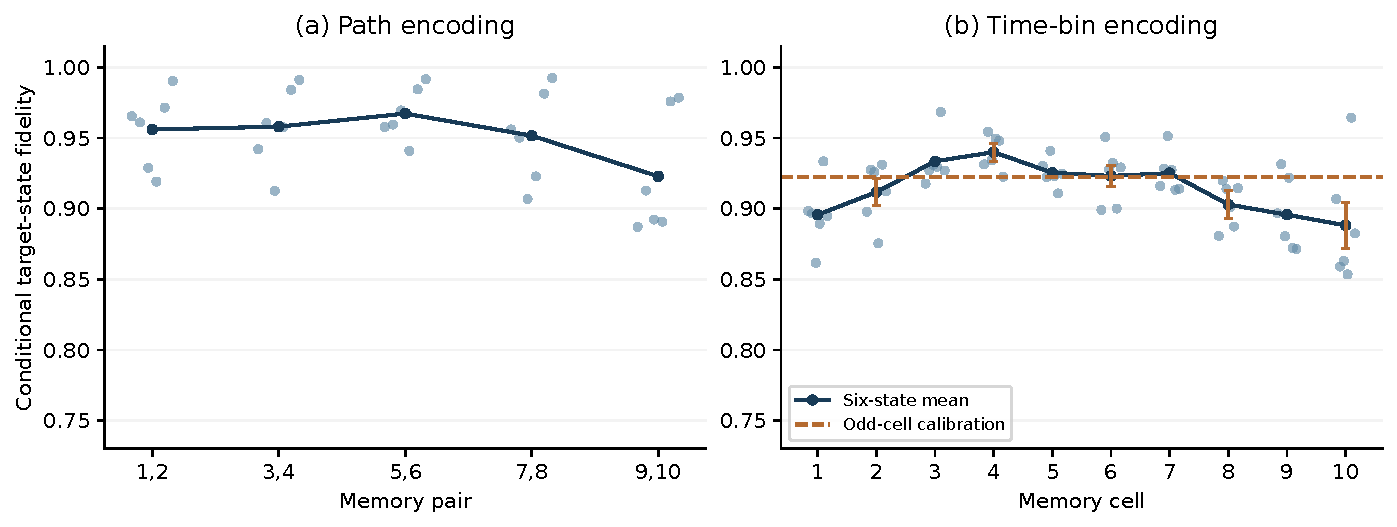
\includegraphics[width=\linewidth]{figures/teller_fidelities.pdf}
\caption{Reanalysis of processed data from Teller et al.~\cite{tellerdata}. Small points show the six state fidelities; dark markers show their uniform means. In panel (b), the dashed line is the inverse-variance calibration on odd-numbered cells, and error bars on even cells show supplied MC uncertainties. Conditioning, encodings and the spatial holdout are distinct. Error bars do not include shared systematic uncertainty.}
\label{fig:teller}
\end{figure}

The odd-cell calibration gives $\widehat F=0.9224361$ with an approximate calibration uncertainty 0.0038484. The maximum held-out standardized discrepancy is 2.3417, below the diagnostic threshold. Figure~\ref{fig:teller} shows that passing this check is compatible with visible cell variation. It does not establish microscopic material uniformity.

We also fit fidelity versus \emph{detection-window width} at fixed storage age. A finite Gaussian pulse with flat unpolarized background has
\begin{equation}
F(w)=\tfrac12+(F_s-\tfrac12)
\frac{\operatorname{erf}(w/(\sqrt8\sigma_p))}
{\operatorname{erf}(w/(\sqrt8\sigma_p))+bw},
\label{eq:window}
\end{equation}
with consistent time units. Calibration uses 80 widths at or below 600~ns; assessment uses 91 widths at or above 800~ns; 40 intermediate widths are unused. The three maximum held-out pointwise discrepancies are 1.729, 2.638 and 0.723. The corresponding constant-fidelity diagnostics have discrepancies 5.547, 5.279 and 4.119 and are flagged as mismatches. One fitted signal fidelity reaches its upper bound. Nested windows share counts, so these are pointwise adequacy diagnostics rather than independent statistical validation; Eq.~\eqref{eq:window} does not estimate $T_2$.

\subsection{A finite operating-point channel and its network control}
For path pair 5,6 and a 270~ns detection window, the reviewed point has conditional six-state mean $F_0=0.9671968089$ and supplied MC uncertainty 0.0051670. The reported cryostat temperature is 3~K; the optical input-to-output time is 18~$\mu$s, comprising 10~$\mu$s AFC rephasing and 8~$\mu$s spin storage. These are distinct from the detection-window width.

The chosen isotropic approximation is
\begin{equation}
\Phi_p(\rho)=(1-p)\rho+pI/2,\qquad p=2(1-F_0).
\label{eq:point}
\end{equation}
This is one effective model calibrated to the mean, not a channel inferred uniquely from process tomography. The derived signal-acceptance model is
\begin{equation}
\eta_0=0.16\times0.42\times0.50\times0.42=0.014112,
\end{equation}
combining AFC efficiency, two-way optical transfer, demultiplexing and temporal acceptance. The propagated component uncertainty is 0.0015824 under independent component errors and exact temporal acceptance. Transfer measurements use classical light; acceptance uncertainty and covariance are unavailable. Fiber coupling, filters, detectors and analysis success are outside this loss model. The simulation therefore does not reproduce a measured complete single-photon network efficiency.

Analytical and QuTiP Choi matrices at this point agree to $1.21\times10^{-17}$. For two identical conditional depolarizing channels on an ideal Bell input,
\begin{equation}
F_B=\frac{1+3(1-p)^2}{4}=0.9048185746,\qquad
P_{\rm pair}=\eta_0^2=1.99148544\times10^{-4}.
\end{equation}
SeQUeNCe produces 20, 32, 24 and 11 retrieved pairs for seeds 20261010--20261013, respectively: 87 in 400,000 attempts. The pooled fraction is $2.175\times10^{-4}$ with Wilson 95\% interval $[1.76350,2.68249]\times10^{-4}$, containing the fixed-loss expectation. Maximum joint-density discrepancy from the analytical result is $1.11\times10^{-16}$. Figure~\ref{fig:network} reports Monte Carlo uncertainty only. The same assumptions give a simulated rate 0.2175~s$^{-1}$ over 400~s of combined attempt time; this is not a measured network rate or a validation of its missing optics.

\begin{figure}[tbp]
\centering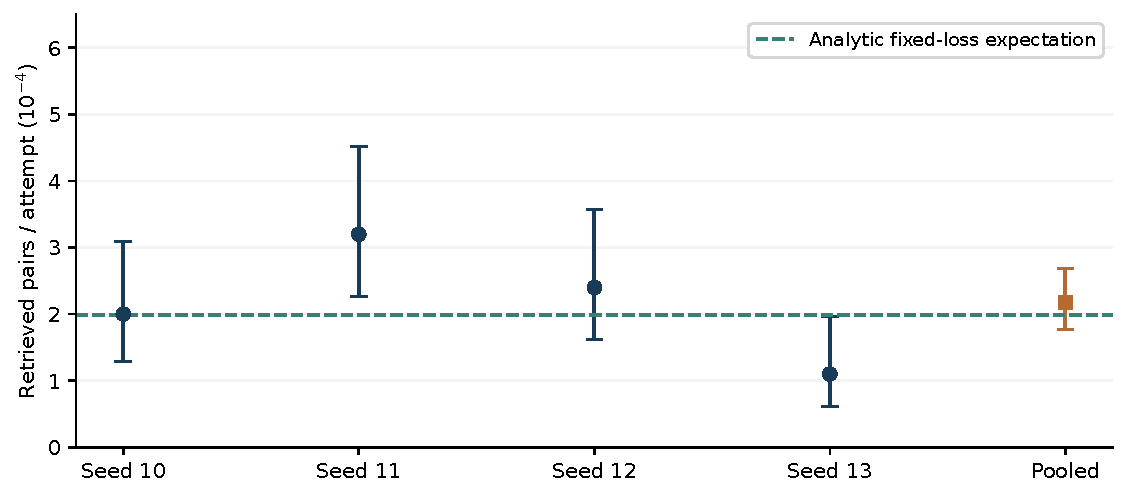
\includegraphics[width=.86\linewidth]{figures/network_control.pdf}
\caption{Ideal-input network integration control for the calibrated, nonunique Teller operating-point model. Individual seeds each use 100,000 attempts; the pooled point uses 400,000. Bars are Wilson intervals from retrieval counts under fixed parameters. Agreement with the analytical loss model verifies implementation; uncertainty in the optical parameters and false-herald physics is not included.}
\label{fig:network}
\end{figure}

An additional constructive calculation makes the mean-only limitation explicit. A phase-flip channel with probability $q=3p/4$ has the same average fidelity as Eq.~\eqref{eq:point}, but two such channels yield a different Bell fidelity. The Supplement records the exact matrices and numerical values. This example concerns the mean constraint alone; it does not assert that both models fit every released state or density matrix.

\subsection{Failure of simple decay models on the second experiment}
Figure~\ref{fig:decay} shows the released efficiency curves and the two tested envelopes. All six RF-curve/model combinations are flagged as model mismatches under the declared Gaussian-error diagnostic. XX held-out RMSE values are 3.582 (exponential) and 2.853 (stretched); XY4 values are 3.786 and 3.434; XY16 values are 1.983 and 1.417. The latter two pass the held-out RMSE screen but fail the full-data goodness-of-fit diagnostic. The source paper itself discusses nonexponential behavior~\cite{rodriguez}; our analysis verifies that the simple diagnostic path does not turn those curves into an unsupported homogeneous lifetime.

\begin{figure}[tbp]
\centering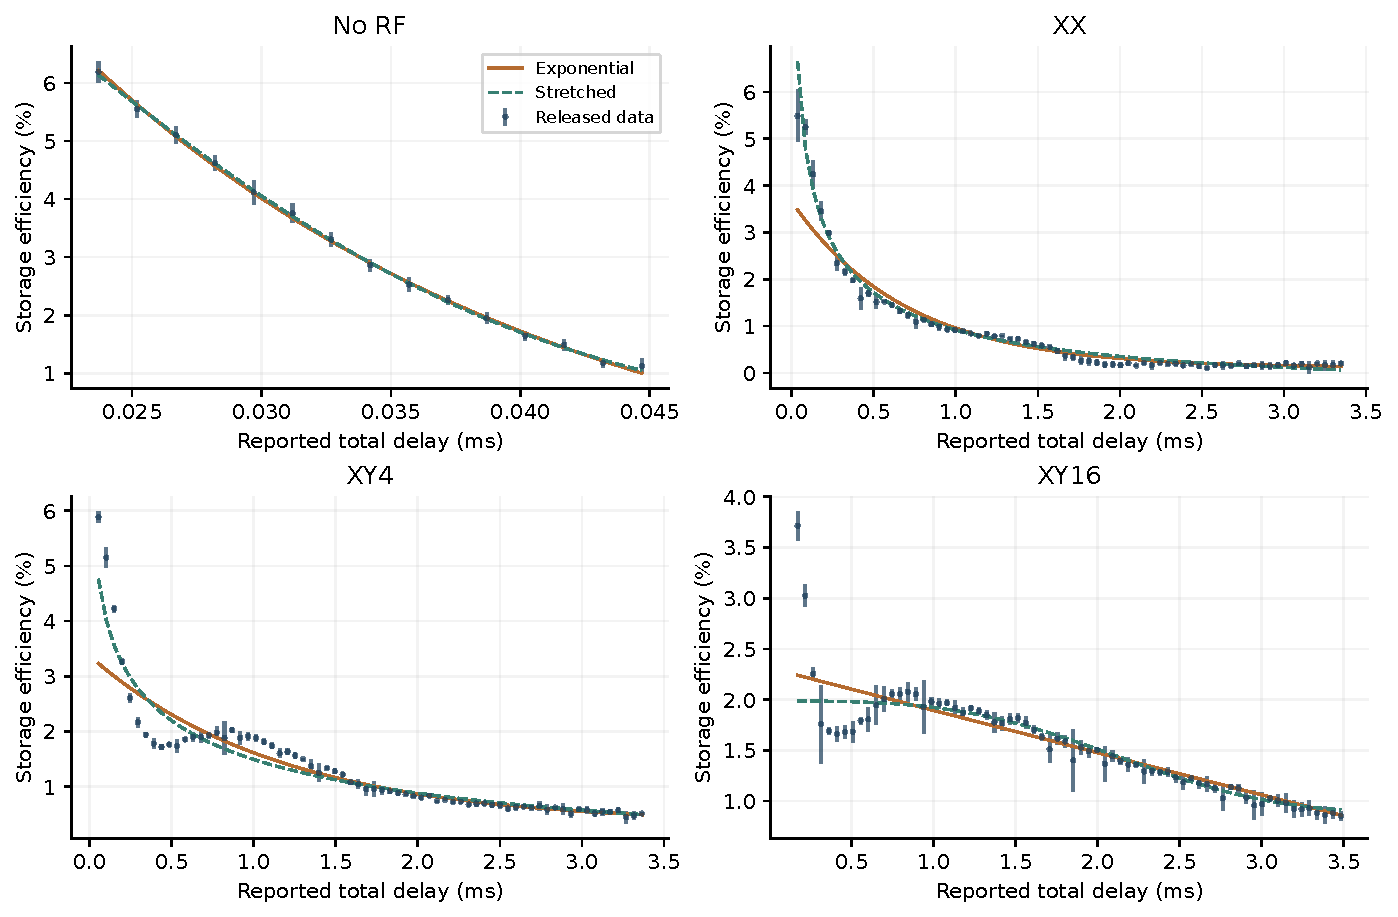
\includegraphics[width=\linewidth]{figures/pr_decay_diagnostics.pdf}
\caption{Processed open classical-efficiency data~\cite{prdata} and diagnostic fits with Eq.~\eqref{eq:curve}. Three RF curves have 70 observations each; the no-RF curve has 15. Curves are plotted against the source's reported total delay. Error bars are the released uncertainties. Fits are apparent retrieval envelopes, not inferred spin-$T_2$ curves. The panels have different horizontal scales.}
\label{fig:decay}
\end{figure}

The no-RF exponential fit returns an apparent scale outside its observed interval; the stretched fit has insufficient stable bootstrap draws. Both are inconclusive. No fit in this case returns an identified physical spin $T_2$. Reported tiny Gaussian goodness-of-fit probabilities condition on independence and the supplied error model; they are not evidence for a unique microscopic cause of the mismatch. Modulations, noise, field uncertainty and protocol details require additional modeling. The withheld heralded-photon arrays also do not measure qubit fidelity, so they cannot repair that missing identification by themselves.

\subsection{Deterministic controls and condition-sensitive references}
For the supplied Markov control, $\Gamma_1=10$~s$^{-1}$ and $\Gamma_\phi=20$~s$^{-1}$ give $T_2=40$~ms at its declared hypothetical conditions. Independent parameter-box ranges $[8,12]$ and $[18,22]$~s$^{-1}$ produce $T_2\in[35.714,45.455]$~ms. Four corner evaluations implement this range. Its relative deviation is $-10.71\%/+13.64\%$ about the nominal value; this is deterministic interval propagation, not prediction accuracy or a statistical confidence interval.

The one-nucleus bath control specifies $I=1/2$, central projections $\pm1/2$, longitudinal hyperfine coupling $A_{zz}=4$~kHz and $T=4.2$~K. For the high-temperature unpolarized limit, $L(t)=\cos(\pi A_{zz}t)$. The finite-temperature implementation uses the Gibbs state exactly. Free evolution has revivals and a first sampled $1/e$ crossing bracket of 90--100~$\mu$s. An ideal Hahn pulse refocuses the commuting longitudinal coupling, with no sampled crossing up to 1~ms. These are software controls, not predictions for a newly selected molecule.

\begin{figure}[tbp]
\centering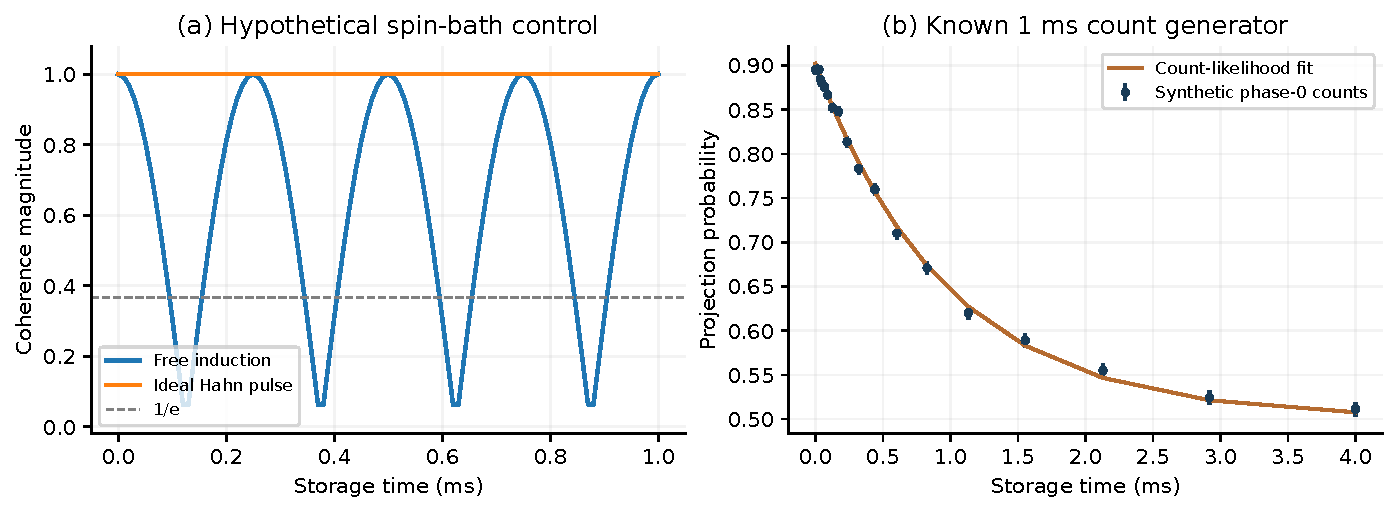
\includegraphics[width=\linewidth]{figures/deterministic_controls.pdf}
\caption{Explicitly synthetic verification cases. (a) Supplied one-nucleus Hamiltonian under free evolution and ideal Hahn refocusing; a finite bath can revive and need not have an exponential lifetime. (b) Phase-zero projections from the four-phase binomial control and fitted probabilities. All phases, rather than only the displayed phase, enter the likelihood.}
\label{fig:controls}
\end{figure}

The count control recovers 0.979663~ms from the known 1~ms generator, with a conditional parametric-bootstrap 95\% interval of [0.950215,1.007737]~ms. Recovery in one synthetic instance checks the likelihood implementation; it is not a coverage study or evidence for physical prediction accuracy. All phases at a held-out age remain outside the holdout fit.

The reviewed table query returns the 230~ms Eu/YSO XY16 effective-spin reference under its reported matching conditions~\cite{ortu}. An unknown-material query yields no applicable reference; changing a required temperature also prevents a match. Ten reviewed rows and 201 provisional molecular observations coexist without sharing the same physical-usability status. Three deterministic specifications, 202 bath-time evaluations and four rate-box corners are recorded, alongside the eight experimental curve-model fits.

The separate hypothetical network control runs SeQUeNCe for 2000 attempts and retrieves 321 pairs. QuTiP/analytical full-channel Choi difference is $4.00\times10^{-15}$ and maximum retrieved-density discrepancy is $5.55\times10^{-17}$. These are checks of supplied write/store/read parameters, distinct from the experiment-constrained point above. The complete automated suite passes 75 tests, covering units, channels, bath dynamics, adapters, source handling, reference restrictions and workflow behavior.

\section{Discussion}
The executed results support the framework's ability to preserve distinctions that matter physically. It reproduces published processed-data summaries, constructs a conditional point model with explicit ambiguity, carries that model into an actual event simulator, and withholds physical lifetimes when its data or model are insufficient. The negative outcomes are part of the evidence: the constant readout-window model is inadequate, the simple RF-decay models mismatch, and an unknown material has no table-derived lifetime.

The results do not validate an arbitrary chain from electronic structure to phonon relaxation to optical memory fidelity. Such a chain needs experimentally anchored Hamiltonians, bath and phonon parameters, pulse errors, sample thermometry, optical coupling and a detection/noise instrument. Reproducing a processed mean does not reconstruct raw trials; a spatial holdout within one dataset does not supply independent hardware replication; numerical Choi agreement does not compensate for omitted physics. Several reference values come from each study, and many molecular entries share source papers, so row counts should not be interpreted as independent sample sizes.

The main implementation boundary is useful even for negative candidate outcomes. Structural or charge/isotope variations can be enumerated and supplied to the appropriate solver. If an optical interface is unknown, coherence can be studied under explicit assumptions while device usability remains unresolved. If the dynamical model shows revivals or a short-window fit is unidentifiable, the output can preserve the curve or bounds instead of forcing a single rankable number. No chemical combination is labeled experimentally new merely because it is absent from the local database.

There are also limitations at the software level. The family taxonomy is finite, bath dimension is bounded, classical propagation is not automatically promoted to a single-photon instrument, and exported histories have fixed control and exact-age semantics. State-dependent heralding, intervention-dependent non-Markovian histories, thermal ramps, realistic generation/detection and additional simulator engines require new validated contracts. NetSquid and QuISP were not run; agreement between QuTiP, an analytical map and SeQUeNCe is not a two-network-simulator cross-validation study. Runtime and scaling on a cluster or supercomputer were not benchmarked. Adapter availability should therefore not be mistaken for validated microscopic coverage of all elements and molecules.

Next validation should use time-resolved fidelity, success and noise at the same storage times, with raw counts, preparation/analysis settings, photon statistics and covariance. Realistic spin-bath applications need independent parameter review and convergence over bath size, cluster order and pulse resolution. A matched benchmark in a second network simulator would then test event semantics separately from channel approximation. These additions would broaden the system's validated scope, regardless of whether a new candidate improves performance.

\section{Reproducibility and availability}
The companion repository bundle includes the evaluated Python source, configurations, cached evidence, figure-generation script, machine-readable results, source/claim mappings and Supplement. The base software archive is identified by SHA-256
\par\noindent\begin{minipage}{\linewidth}\centering\small
\texttt{c64b94a573def9d999b65be7201947e9c}\\
\texttt{2ce4e496aaf201650d7c1e3d44733aa}
\end{minipage}\par
The manuscript's headline results were freshly reproduced from that archive's source. No public software DOI or repository URL is asserted; the deliverable is a local repository-ready bundle. External experimental datasets retain their original DOIs~\cite{tellerdata,prdata}. Third-party source and data notices accompany the bundle, and cached source files are excluded from the default Git tracking rules. The independently maintained ML project is not included as a dependency.

The tested runtime is Python 3.12.14, NumPy 2.5.3, SciPy 1.18.1, QuTiP 5.3.1, PySCF 2.14.0, PyCCE 1.1.1 and SeQUeNCe 1.2.0 on Linux. Dependency constraints and actual logs are archived. A container compatibility fallback for PySCF reads the same RSS/VMS page counts through \code{/proc/self/statm} when numeric PID paths are unavailable; it does not change an electronic-structure equation. The Supplement provides the exact commands, seeds, uncertainty assumptions and result files. AI-assisted coding and drafting were used; these tools are not credited as authors, and scientific responsibility remains with the named author.

\section{Conclusion}
WestQuant Memory Discovery Lab provides an executable, evidence-aware route from heterogeneous source data to scoped quantum-memory observables and optional channel-based network simulation. Open experimental reanalysis, within-dataset diagnostics and independent numerical checks support specific parts of that route. The evaluated framework deliberately leaves unsupported lifetimes and new-material performance unresolved. Its present contribution is a reproducible integration with explicit physical and evidential boundaries, rather than a demonstrated improvement in a material or a fully validated universal memory simulator.

\begin{thebibliography}{99}
\bibitem{teller} M. Teller, S. Plascencia, S. Grandi and H. de Riedmatten, ``Quantum Storage of Qubits in an Array of Independently Controllable Solid-State Quantum Memories,'' \emph{Physical Review X} \textbf{15}, 031053 (2025). \href{https://doi.org/10.1103/z6lc-qw2d}{doi:10.1103/z6lc-qw2d}.
\bibitem{tellerdata} M. Teller et al., ``Supporting data of Quantum storage of qubits in an array of independently controllable solid-state quantum memories,'' Zenodo record 14929997 (2025). \url{https://doi.org/10.5281/zenodo.14929997}.
\bibitem{ortu} A. Ortu, A. Holz\"apfel, J. Etesse and M. Afzelius, ``Storage of photonic time-bin qubits for up to 20 ms in a rare-earth doped crystal,'' \emph{npj Quantum Information} \textbf{8}, 29 (2022). \url{https://doi.org/10.1038/s41534-022-00541-3}.
\bibitem{rodriguez} E. Rodr\'iguez-Moldes et al., ``Long-Lived Telecom-Heralded Single-Photon Storage in an Absorptive Spin-Rephased Quantum Memory,'' \emph{Physical Review Letters} \textbf{137}, 120803 (2026). \url{https://doi.org/10.1103/ftkb-pkvp}. Author manuscript: arXiv:2609.02579v1.
\bibitem{prdata} E. Rodr\'iguez-Moldes et al., ``Dataset from Long-lived telecom-heralded single-photon storage in an absorptive spin-rephased quantum memory,'' Zenodo record 21532904 (2026). \url{https://doi.org/10.5281/zenodo.21532904}.
\bibitem{lin} C.-Y. Lin, T. Ngendahimana, G. R. Eaton, S. S. Eaton and J. M. Zadrozny, ``Counterion influence on dynamic spin properties in a V(IV) complex,'' \emph{Chemical Science} \textbf{10}, 548--555 (2019). \url{https://doi.org/10.1039/C8SC04122A}. Primary full text: PMCID PMC6335635.
\bibitem{mullin} K. R. Mullin, D. Johnson, D. E. Freedman and J. M. Rondinelli, ``Systems-chart approach to the design of spin relaxation times in molecular qubits,'' \emph{Dalton Transactions} \textbf{53}, 16585--16591 (2024). \url{https://doi.org/10.1039/D4DT02311K}.
\bibitem{mtd} MTD-group, \emph{Molecular Qubit Dataset}, source revision 5263b1d86b39243e7405dde5bf7c58bbd8fcd677, accessed 10 October 2026. \url{https://github.com/MTD-group/Molecular_Qubit_Dataset}.
\bibitem{hu} H. Hu et al., ``Room-temperature waveguide integrated quantum register in a semiconductor photonic platform,'' \emph{Nature Communications} \textbf{15}, 10256 (2024). \url{https://doi.org/10.1038/s41467-024-54606-2}.
\bibitem{pyscf} Q. Sun et al., ``Recent developments in the PySCF program package,'' \emph{Journal of Chemical Physics} \textbf{153}, 024109 (2020). \url{https://doi.org/10.1063/5.0006074}.
\bibitem{pycce} M. Onizhuk and G. Galli, ``PyCCE: A Python Package for Cluster Correlation Expansion Simulations of Spin Qubit Dynamics,'' \emph{Advanced Theory and Simulations} \textbf{4}, 2100254 (2021). \href{https://arxiv.org/abs/2107.05843}{arXiv:2107.05843}; \href{https://doi.org/10.1002/adts.202100254}{doi:10.1002/adts.202100254}.
\bibitem{qutip} N. Lambert et al., ``QuTiP 5: The Quantum Toolbox in Python,'' \emph{Physics Reports} \textbf{1153}, 1--62 (2025). \href{https://arxiv.org/abs/2412.04705}{arXiv:2412.04705}.
\bibitem{maxwellbloch} T. P. Ogden, \emph{MaxwellBloch}, software and official documentation, version used: 0.12.0. \url{https://github.com/tpogden/maxwellbloch}; \url{https://maxwellbloch.readthedocs.io/}.
\bibitem{sequence} X. Wu, A. Kolar, J. Chung, D. Jin, T. Zhong, R. Kettimuthu and M. Suchara, ``SeQUeNCe: a customizable discrete-event simulator of quantum networks,'' \emph{Quantum Science and Technology} \textbf{6}, 045027 (2021). \url{https://doi.org/10.1088/2058-9565/ac22f6}.
\bibitem{aiida} S. P. Huber et al., ``AiiDA 1.0, a scalable computational infrastructure for automated reproducible workflows and data provenance,'' \emph{Scientific Data} \textbf{7}, 300 (2020). \url{https://doi.org/10.1038/s41597-020-00638-4}.
\bibitem{chung} J. Chung et al., ``Cross-Validation of Open-Source Quantum Network Simulators,'' arXiv:2610.09322v1 (2026). \url{https://arxiv.org/abs/2610.09322}.
\end{thebibliography}
\end{document}
